\section{An Adaptive Local Timestepping Algorithm}
\label{sec:alg}
The previous proofs dealt with certain classes of event traces and demonstrated that they were TVD. In this section, we present an algorithm that generates an event trace satisfying the hypotheses of Theorem \ref{thm:tvd-stab}. To allow for an efficient implementation, we couch the algorithm in the language of discrete event simulations, which will allow us to rely on the extensive work done in that field for the parallelization. The main result of this section will demonstrate that with a sufficiently small minimum timestep, our algorithm will generate a total variation stable event trace.

\subsection{Discrete Event Simulation}
Discrete event simulation as a tool has been used extensively for the simulation of numerous phenomena~\cite{Fujimoto1990}. Fundamentally, the simulation is represented as a set of actors denoted here as $\mathcal{A}$, and a set of events to be executed on an actor at a given point in time. When executed, each event may then schedule more events with later timestamps. The discrete event simulator guarantees that events will be executed in order of their timestamps.
%\Cy{It's probably worth mentioning here that we use sub-times to schedule multiple events at the same $\tau$ timestamp.}

At a high level, the actors used for the approximation of solutions to conservation laws will consist of submeshes. For this section, we require that at least two elements be assigned to each submesh. However, given an update rule with a $2n+1$-sized stencil per cell as is the case for high order finite volume methods, we require that the submesh contain at least $n+1$ cells. In practice, achieving performance requires balancing the overhead of the simulator against the amount of useful work being done during each task~\cite{Bremer2019}. Therefore, submeshes should contain significantly more cells to balance simulation overheads. Each submesh can schedule one of two events: (1) {\em Update} ($\mathcal{U}$) the submesh to the time at which the update is scheduled, and (2) {\em Push Flux} ($\mathcal{PF}$), wherein the submesh sends relevant metadata to the neighboring cell to allow advancing along the shared boundary. We quantize our time to be an integer multiple of a smallest timestep, $\Delta t_{\min}$. In this section, we use $t,\,\tprev,\,\tnext$ as variable names and $\tau$ is used to specify timestamps in the discrete event simulation.

\begin{figure}
\centering
\subfloat[Submesh class\label{class:submesh}]{\usebox{\submeshlisting}}\hspace{2in}
\subfloat[Interface class\label{class:interface}]{\usebox{\interfacelisting}}
\caption{Local timestepping data structures}
\end{figure}

The actor states are described in Figure~\ref{class:submesh}. The actor's members correspond to
\begin{itemize}
\item $id$: The submesh id,
\item $t$: The current time of the submesh,
\item $\tprev$: The last time at which the submesh was updated,
\item $\tnext$: The next time at which the submesh is scheduled to be updated,
\item $u$: The average density on each cell,
\item $\Delta x$: The sizes of the cells for the submesh,
\item $\ell,\,r$: Representations of the states to the left and right of the submesh, respectively. 
\end{itemize}
The interface class in Figure~\ref{class:interface} describes neighboring cell metadata and has members describing: %\Max{Description of K confusing} %\Cy{Consider using a different symbol for the $\tprev$ in the interface vs the $\tprev$ in the actor}
\begin{itemize}
\item $id$: The id of the neighboring submesh,
\item $\tprev$: The last time at which the neighbor was updated,
\item $\tsync$: The last time at which the neighbor and submesh both updated,
\item $u$: The neighbor's density at time $\tprev$,
\item $K^*$: The largest Lipschitz constant of the numerical flux between time $\tsync$ to $\tprev$ on the internal interface ($K^{\intr}$) or external interface cell ($K^{\extr}$),
\item $\Sigma \hat{F}$: The integral of the numerical flux between the submesh and its neighbor from time $\tprev$ to the current time,
\item $\Delta x$: is the size of the neighboring cell.
\end{itemize}
We note that the Lipschitz constant $K$ is used to bound $C_j$ and $D_j$ terms simultaneously. For commonly used fluxes like the Godunov flux or Lax-Friedrichs flux, $K$ will look like $|\Lambda|/\Delta x$ yielding the commonly seen version of the CFL condition \eqref{eq:vanilla-cfl}.
Member fields are denoted using a period, e.g. $S.\ell.\tprev$ denotes the previous update of the left interface of submesh $S$.
We next turn to describing our events. Before we define our two main events, {\sc update} and {\sc push\_flux}, we define some helper functions.
\begin{definition}[Helper Functions]
\label{def:helper-functions}
\begin{itemize}
\item {\sc advance(t, submesh)}: Advance the submesh one timestep from submesh.$\tprev$ to $t$ according to the update rule~\eqref{eq:update}. Note that this will also cause corresponding updates in boundary terms such as $K^*$ and $\Sigma \hat{F}$.
\item {\sc compute\_t\_next\_bdry(submesh, neigh)}: Compute the timestep size for interfaces which depend on neigh.$u$. This evaluates two CFL conditions at: (1) the external interface between the submesh and its neighbor, which is synchronized at neigh.$\tsync$ and (2) the internal interface nearest to the external interface, which is synchronized at submesh.$\tprev$.
\item {\sc compute\_t\_next(submesh, t)}: Compute the allowable timestep size for the submesh. This is taken to be the minimum of the largest timesteps for the values returned by {\sc compute\_t\_next\_bdry} for both neighbors and the largest allowable internal timestep.
\item {\sc make\_msg(submesh, neigh)}: Generate a buffer with the required information to update the neighbor's corresponding interface.
\item {\sc accumulate(t, submesh, neigh)}: Update neigh.$\Sigma \hat{F}$ to integrate from the previous integration point neigh.$\tprev$ to time $t$. 
\item {\sc update\_K\_bdry(submesh, neigh)}: Update Lipschitz constants $K^*$ according to the new updated values at the boundary.
\end{itemize}
\end{definition}
The helper functions serve as an API between the application and the timestepping algorithm. Features like which set of conservation laws or choice of discretization are encapsulated into the above function calls. In addition to the helper functions, we also define our scheduling primitives. These are the function calls with which events are scheduled in the discrete event simulator.

\begin{definition}[Scheduling Primitives]
\label{def:scheduling-primitives}
\begin{itemize}
\item {\sc schedule(t, event)}: Schedule {\sc event} at time {\sc t} in the discrete event simulator.
\item {\sc schedule\_inline(event)}: Execute {\sc event} in the current execution context, i.e. on that actor at that time.
\end{itemize}
\end{definition}

\begin{figure}
\begin{lstlisting}[mathescape=true, basicstyle=\scriptsize]
function update(id, update_forced)
  $\tau \gets$ get_time()
  submesh $\gets$ get_submesh(id)

  if ( $\tau \neq \text{submesh}.\tnext \land \neg \text{force\_update}$ ) return
  if ( $\tau = \text{submesh}.\tprev$ ) return
    
  advance($\tau$, submesh)
  submesh.$\tnext$ $\gets$ compute_t_next(submesh, $\tau$)
  
  for neigh $\in$ submesh.bdry
    forced_update $\gets$ neigh.$\tprev$ > neigh.$\tsync$
                  $\land$ compute_t_next_bdry(submesh, neigh) $\le \tau$
                  
    schedule( $\tau$, push_flux( neigh.id, id,
                            make_msg(submesh, neigh),
                            force_update) )
    if ( forced_update ) neigh.$\tsync$ $\gets\tau$
    
  if ( submesh.$\tnext > \tau$ )
    schedule(submesh.$\tprev$, update(id, false))
\end{lstlisting}
\caption{Update function}
\end{figure}

\begin{figure}
\begin{lstlisting}[mathescape=true,basicstyle=\scriptsize]
function push_flux(id, id_from, msg, force_update)
  $\tau \gets$ get_time()
  submesh $\gets$ get_submesh(id)
  neigh $\gets$ get_neigh(submesh, id_from)
  
  accumulate( $\tau$, submesh, neigh )
  neigh.u $\gets$ msg
  neigh.$\tprev$ $\gets \tau$
  if ( neigh.$\tprev =$submesh.$\tprev$ ) neigh.$\tsync$ $\gets \tau$
  update_K_bdry(submesh, neigh)
  
  submesh.$\tnext$ $\gets$ compute_t_next(submesh, $\tau$)
  if ( force_update $\lor$ submesh.$\tnext \le \tau$ )
    schedule_inline(update(id, true))
    return
    
  if ( submesh.$\tnext > \tau$ )
    schedule(submesh.$\tnext$, update(id, false))
\end{lstlisting}
\caption{Push flux function}
\end{figure}

With these helper functions, we now define our two main events: update ($\update$) and push flux ($\pushflux$). Shown in Algorithm~\ref{alg:des}, the main loop schedules initial updates at time 0 in a priority queue ($\pq$). As events execute, they may cause other events to be enqueued in the priority queue as pairs with the desired timestamp of evaluation as the key. The lowest timestamps receive the highest priority, and in case of ties, we impose no ordering.

\begin{algorithm}
\caption{Main timestepping loop}\label{alg:des}
\begin{algorithmic}
\State Initialize actors $\mathcal{A}= \{ S_1,\ldots, S_{n_{sbmsh}} \}$
\State Initialize $\pq := \{\}$
\For{$sbmsh \in \mathcal{A}$}
  \State schedule( 0, update($sbmsh.id$, false))
\EndFor

\While{$\exists\,q \in \pq$}
  \State current\_event $\gets \pq$.pull\_highest\_priority()
  \State evaluate(current\_event)
\EndWhile
\end{algorithmic}
\end{algorithm}

We now arrive at the main result for this section.
\begin{theorem}
\label{thm:des-tvd}
Given a minimum timestep size of
\begin{equation}
\Delta t_{\min} < \inf\left\{ \frac{\Delta x_{\min}}{2 \max(K_1(\xi),\,K_2(\xi))}\, : \, \xi \in \range(u_0) \right\},
\label{eq:dt-min}
\end{equation}
where $\Delta x_{\min}$ is the smallest element size, $K_1(\xi)$ is the local Lipschitz constant of $\hat{F}(\cdot,\xi)$ and $K_2(\xi)$ is the local Lipschitz constant of $\hat{F}(\xi,\cdot)$. The discrete event simulator as defined in Algorithm \ref{alg:des} with a minimum timestep of $\Delta t_{\min}$ will produce a TVD solution to the scalar conservation law in~\eqref{eq:ivp}.
\end{theorem}

\subsection{Proof of Theorem \ref{thm:des-tvd}}
The proof of the theorem requires demonstrating that the discrete event simulation generates an event trace that satisfies the conditions of Theorem~\ref{thm:tvd-stab}. The main machinery for this proof will be loop invariants. Loop invariants are a formal correctness technique whereby we specify a set of ``correct'' states. By showing that every event maps a correct state onto the set of correct states, we are able to ensure that the following state satisfies certain desired criteria. Once all events have executed, we will have proven that the simulation terminates in the correct state and the algorithm behaves as desired. This proof technique has been utilized with great success for systematic design of algorithms for numerical linear algebra as part of the FLAME project~\cite{Bientinesi2011, Myers2018}.
 To demonstrate that the algorithm satisfies the conditions of Theorem~\ref{thm:tvd-stab}, we need invariants to satisfy:
\begin{enumerate}
\item the local ordering principle,
\item the CFL condition,
\item and the update rule as expressed in \eqref{eq:update}.
\end{enumerate}
Additionally, we will require two further invariants to show that the computed values are correct, and that duplicated metadata in the boundaries is consistent with the values on the neighboring submesh. To simplify, the notation in these invariants, we assume three submeshes are enumerated as, $S_A$, $S_B$, and $S_C$. The value of $u$ at the cell neighboring another submesh, will be indexed with that neighbors name, e.g. the cell in submesh $S_B$ that neighbors $S_A$ we will reference as $S_B.u_A$. For clarity, we have depicted this naming convention in Figure~\ref{fig:submeshes}.
\begin{figure}
\centering
  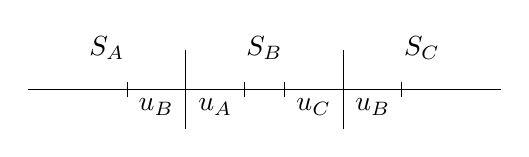
\begin{tikzpicture}
    \draw (-3,0)-- (-1,0) node[midway, above, label={[distance=1cm]:$S_A$}] {};
    \draw (-1,0)-- ( 1,0) node[midway, above, label={[distance=1cm]:$S_B$}] {};
    \draw ( 1,0)-- ( 3,0) node[midway, above, label={[distance=1cm]:$S_C$}] {};
    \draw (-1,-0.5)--(-1,0.5);
    \draw ( 1,-0.5)--( 1,0.5);
    \draw[|-] (-1.75,0)--(-1,0) node[midway,below] {$u_B$};
    \draw[-|] (-1,0)--(-0.25,0) node[midway,below] {$u_A$};
    \draw[|-] ( 0.25,0)--( 1,0) node[midway,below] {$u_C$};
    \draw[-|] ( 1,0)--( 1.75,0) node[midway,below] {$u_B$};
  \end{tikzpicture}
\caption{Three neighboring submeshes $S_A,\,S_B,$ and $S_C$ with bordering cells named.}
\label{fig:submeshes}
\end{figure}
% \Cy{consider more clearly defining the term "synchronization time" at or before this point}\Max{This is introduced in the first order method section.}


Local ordering implies that one of two neighboring submeshes must have last updated at the last synchronization time.  To ensure that the event trace will be locally ordered, we define the local ordering invariant for the left interface as
\begin{align}
LO_{\ell}(S_B,\tau) &= (S_B.\tprev = S_B.\ell.\tsync\,\lor\,S_B.\ell.\tprev = S_B.\ell.\tsync) \label{eq:LO1}
\end{align}
%\Cy{This is the first use of $\tau$ I found in this section.  I think I figured it out: $\tau$ is just a particular time you're evaluating the invariants, and the various $t$s are used as variable names.}
Note that we similarly define $LO_r(S_B,\tau)$ for the right interface. The $\tau$ in the arguments of the loop invariants refers to the simulation time at which we evaluate the invariant.

Next, we define the CFL-related invariants. These invariants will ensure that our algorithm satisfies the CFL condition~\eqref{eq:cfl-tvd}. Define the invariant for the left boundary cell as
\begin{align}
CFL_{\ell}(S_B, \tau) &= ( S_B.\tnext - S_B.\ell.\tsync) S_B.\ell.K^{\extr} \le 1/2 \label{eq:CFL:ext}\\
& \land\, (S_B.\tnext - S_B.\tprev) S_B.\ell.K^{\intr} \le 1/2, \label{eq:CFL:int}
\end{align}
where $K$ is used to bound the respective $C_j$ and $D_j$ terms. Note that \eqref{eq:CFL:ext} corresponds to interface between submeshes $S_A$ and $S_B$, thus the CFL condition is relative to $S_B.\ell.\tsync$. The other CFL condition \eqref{eq:CFL:int} corresponds to the interior interface of the cell associated with $S_B.u_a$. Since internally the internal cells step synchronously, the last synchronization time is $S_B.\tprev$, but since $S_B.\ell.K^{\intr}$ still depends on $S_B.\ell.u$, this condition must be re-evaluated after each push flux. We  define a CFL invariant for the right interface, $CFL_r(S_B, \tau)$ similarly. We also define an internal CFL invariant, $CFL_{\intr}$, which can be determined by solely examining the internal state of the submesh.
\begin{equation*}
    CFL_{\intr} = \bigwedge_{i=2}^{n_{el-1}} \big( (S_B.\tnext - S_B.\tprev) \big[D_i(S_B.u_{i-1},S_B.u_i, S_B.u_{i+1}) - C_i(S_B.u_{i-1},S_B.u_i,S_B.u_{i+1})\big] \le 1 \big)
\end{equation*}
We then define our CFL invariant as
\begin{equation}
CFL(S_B,\tau) =  (CFL_{\intr}\,\land\,CFL_{\ell}\,\land\,CFL_r). \label{eq:CFL:1}
\end{equation}
The correctness invariant $CR$ checks that all computations are being done correctly. Here, we use $\tilde{S}_B$ to denote the state before executing an event.
\begin{align}
CR&(S_B,\tau) = \big( (S_B.\tprev =\tilde{S}_B.\tprev\,\land\,S_B.u = \tilde{S}_B.u) \label{eq:CR1}\\
&\quad\quad\lor (S_B.\tprev \neq \tilde{S}_B.\tprev \,\land\,S_B\text{ updated according to Equation~\eqref{eq:update}} \big)\label{eq:CR2}\\
&\land \left( S_B.\ell.\Sigma \hat{F} = \int_{S_B.\tprev}^{\max(S_B.\ell.\tprev,S_B.\tprev)} \hat{F}(S_B.\ell.u(\sigma), S_B.u_A) \,\mathrm{d}\sigma \right)\label{eq:CR3}\\
&\land \left( S_B.r.\Sigma \hat{F} = \int_{S_B.\tprev}^{\max(S_B.r.\tprev,S_B.\tprev)} \hat{F}(S_B.u_C, S_B.r.u(\sigma)) \,\mathrm{d}\sigma \right)\label{eq:CR4}\\
& \land\,S_B.\ell.K^{\intr} \ge \max_{\sigma \in (S_B.\tprev, \tau)} D_j(S_B.\ell.u(\sigma), S_B.u_A, S_B.u_{A+1})\label{eq:CR5}\\
& \land\,S_B.\ell.K^{\extr} \ge \max_{\sigma \in (S_B.\ell.\tsync, \tau)} -C_j(S_B.\ell.u(\sigma), S_B.u_A, S_B.u_{A+1})\label{eq:CR6}\\
& \land\,S_B.r.K^{\intr} \ge \max_{\sigma \in (S_B.\tprev, \tau)} -C_j(S_B.u_{C-1}, S_B.u_C, S_B.r.u(\sigma))\label{eq:CR7}\\
& \land\,S_B.r.K^{\extr} \ge \max_{\sigma \in (S_B.r.\tsync, \tau)} D_j(S_B.u_{C-1}, S_B.u_C, S_B.\ell.u(\sigma)).\label{eq:CR8}
\end{align}
%\Cy{In (4.13) to (4.16), some $u$ values are not dependent on $\sigma$ because their values are constant over the interval, right?  The reader will probably notice this, but I'm not sure if this is worth mentioning in the text.}
 Equations~\eqref{eq:CR1} and~\eqref{eq:CR2} require that if the state has been updated, $S_B.\tprev$ will reflect that, and that the state is updated according to the update rule. We check that the flux buffers are being correctly integrated at the boundary with \eqref{eq:CR3} and~\eqref{eq:CR4}. The last set of equations \eqref{eq:CR5}--\eqref{eq:CR8} check that the $K$ terms used to enforced the CFL condition correctly bound the Lipschitz constants of the numerical flux. Internal values of $S_B.u$ in \eqref{eq:CR5}--\eqref{eq:CR8} have no dependence on the time variable $\sigma$ since the solution remains constant on a cell between updates. For this invariant to be well-defined, we require that each submesh contain at least two cells. Otherwise, terms like $S_B.u_{A+1}$ would not exist.

The previous three invariants, $LO, CFL,$ and $CR$, have all used information available on submesh $S_B$. However, when duplicating information between neighbors, we need to ensure that the information is consistent. Thus, we define a consistency invariant,
\begin{align}
CI(S_B, S_A, \tau) &= \big( S_B.u_A = S_A.r.u_B \,\land\, S_B.\tprev = S_A.r.\tprev)\label{eq:CI1}\\
&\quad\quad \lor\, \exists\,(\tau,\pushflux(S_A.id, S_B.id, S_B.u_a, \cdot))
\in\pq \big)\label{eq:CI2}\\
&\land\,\big( S_B.\ell.\tsync = S_A.r.\tsync\label{eq:CI3}\\
&\quad \lor\, ( S_B.\ell.\tsync = \tau \,\land\,\exists\,(\tau,\pushflux(S_A.id,S_B.id,\cdot,\cdot))\in \pq\label{eq:CI4}\\
&\quad\lor\, (S_A.r.\tsync=\tau \,\land\,\exists\,(\tau,\pushflux(S_B.id,S_A.id, \cdot, \cdot)) \in \pq \big)\label{eq:CI5}
\end{align}
Here we use the dot, $\cdot$ to denote any argument. Note that we similarly define consistency for the other interface between $S_B$ and $S_C$.

The last invariant we define is a progress invariant to ensure that the simulation can make progress,
\begin{align}
P(S_B, \tau) &= (S_B.\tprev = t_{end})\\
&\lor  (\exists\,(s,\update(s,S_B,false))\in\pq \, :\, \{s = \,S_B.\tnext \ge \tau > S_B.\tprev\})\label{eq:P2}\\
&\lor  \exists\,(\tau, \pushflux(S_B.id, \cdot, \cdot,\cdot))\in \pq \label{eq:P3} \\
&\lor  \exists\,(\tau, \pushflux(\cdot, S_B.id, \cdot, true))\in\pq. \label{eq:P4}
\end{align}
Combining these five loop invariants, we arrive at
\begin{align}
I(S_B, S_A, S_C, \tau) &= LO_{\ell}(S_B) \,\land\, LO_r(S_B) \,\land\,CFL(S_B, \tau) \land CR(S_B, \tau)\\
&\land\,CI(S_B,S_A, \tau) \,\land\, CI(S_B,S_C,\tau)\,\land P(S_B,\tau).
\end{align}

As the aim is to ensure the invariants hold for all submeshes, we will refer to $I(\tau)$ (without the submesh arguments) as
\begin{equation*}
I(\tau) = \bigwedge_{k=1}^{\nsbmsh} I(S_k, S_{k-1}, S_{k+1}, \tau).
\end{equation*}
\begin{proposition}
A discrete event simulation which satisfies the invariant $I$ between all events executed before time $\tau$, will execute a finite number of events at $\tau$ and satisfy $I$ between each of these events.
\label{prop:1step}
\end{proposition}
Assuming Proposition~\ref{prop:1step} holds, the remainder of the proof of Theorem~\ref{thm:des-tvd} follows by induction. At the start of time $\tau$ , we note that no updates have executed, and so $S.\tprev < \tau$. Furthermore, since push fluxes may only be scheduled at the time at which the spawning updates are executed, there are no outstanding push fluxes. Thus, the invariant $I$ before any events have been executed at time $\tau$ is
%\Cy{This might also be a good point to discuss sub-times since we have multiple events executing at a single timestamp.}
%\Cy{use "time" vs "timestamp" consistently}
\begin{align*}
I(\tau, S_B, S_A, S_C) &= LO_{\ell} \,\land\,LO_r\,\land\,CFL_{\intr} \,\land\,CFL_{\ell}\,\land\,CFL_r\,\land\,CR\\
&\land\,S_B.u_A = S_A.r.u_B \,\land\,S_B.\tprev = S_A.r.\tprev\\
&\land\,S_B.\ell.\tsync = S_A.r.\tsync\\
&\land\,S_B.u_C=S_C.\ell.u_B\,\land\,S_B.\tprev =S_C.\ell.\tprev\\
&\land\,S_B.r.\tsync = S_C.\ell.\tsync\\
&\land\,\exists\,(s,\mathcal{U}(S_B.id, false)) \in \mathcal{Q} \text{ for which } \tau \le s \le S_B.\tnext.
\end{align*}
After all events at time $\tau$ have finished executing, we end in the same state, with the exception that the progress invariant implies that every element must have an update scheduled at a time strictly greater than $\tau$. Due to consistency and correctness, every cell which updated at time $\tau$, was updated according to the update rule \eqref{eq:update}. Furthermore, consistency and correctness along with the CFL condition, imply that the event trace up until time $\tau$ satisfies the CFL condition~\eqref{eq:cfl-tvd}. Once all the events have executed, remaining in $I$ implies that updates must be scheduled for time $\tau+\Delta t_{\min}$ or greater, since otherwise the discrete event simulation would not advance past time $\tau$ in a finite number of events. Lastly, the event trace remains locally ordered. Were it not, one of the locally ordered invariants would be violated after all events at $\tau$ had executed. Remarking that the solution remains constant from $\tau$ to $\tau + \Delta t_{\min}$, we have established the inductive hypothesis. Arguing inductively, the event trace at $\tend$ is locally ordered, satisfies the CFL condition, and obeys the forward Euler update rule. Therefore, the discrete event simulation will generate a TVD solution.
%\Cy{$\tau + \Delta t_{\min}$?  I'm still not sure if $\tau$ is in units of seconds or $\Delta t_{\min}$ increments} \Max{Should be \tau + \Delta t_{\min}}


\subsection{Proof of Proposition \ref{prop:1step}}
The remainder of the proof relies on demonstrating that the simulation state satisfies the invariants after each event is evaluated at time $\tau$. However, before we proceed, we prove a progress guarantee.

\begin{proposition}
Given a discrete event simulation that satisfies invariant $I$ up until time $\tau$, $u(\tau)$ will satisfy a maximum principle.
\label{prop:des-max}
\end{proposition}
\begin{proof}
Pick any cell $j$ and consider two update points $t_j^n$ and $t_j^{n+1}$. Let $s_{j-1,j}^{\mu}$ and $s_{j,j+1}^{\eta}$ represent the most recent left and right synchronization times, respectively, and let $u_{j-1}$, $u_j$, $u_{j+1}$ represent the associated cell densities.
Since the total variation CFL condition~\eqref{eq:cfl-tvd} is satisfied for all time up until $\tau$,
\begin{align*}
1 &+ \int_{t_j^n}^{t_j^{n+1}} \big[C_j(\sigma) - D_j(\sigma) \big]\,\mathrm{d} \sigma\\
& \ge 1 + (t_j^{n+1} - s_{j-1,j}^{\mu}) \min_{\sigma \in (s_{j-1,j}^{\mu},t_j^{n+1})} C_j(u_{j-1}, u_j, u_{j+1})\\
& \quad\quad - (t_j^{n+1} - s_{j,j+1}^{\eta}) \max_{\sigma \in (s_{j,j+1}^{\eta}, t_j^{n+1})}D_j(u_{j-1}, u_j, u_{j+1})\\
& \ge 0.
\end{align*}
Thus, the event trace satisfies the maximum principle, Theorem~\ref{thm:max}.
\end{proof}

\begin{lemma}[Progress Guarantees]
\label{lem:progress-guarantee}
Given a simulation that satisfies the invariant $I$ up until time $\tau$, if a submesh $S_B$ and its neighbors $S_A$ and $S_B$ are both updated at time $\tau$, then
\begin{lstlisting}[mathescape=true]
    compute_t_next(submesh, $\tau$) $\ge \tau + \Delta t_{\min}$.
\end{lstlisting}
\end{lemma}
\begin{proof}
Pick any cell of $S_B$ and consider the two neighboring cells. Enumerate the densities as $u_{j-1},\,u_j$ and $u_{j+1}$. 
By definition of the Lipschitz constant
\begin{equation*}
-C_j(u_{j-1}, u_j, u_{j+1}) \le K_1(u_{j+1})/\Delta x_{\min}
\end{equation*}
for all $u_{j-1},\,u_j,\,u_{j+1} \in \range(u_0)$.
By Proposition \ref{prop:des-max}, $u_{j-1}, u_j, u_{j+1} \in \range(u_0)$. Therefore,
\begin{align*}
-\Delta t_{\min} C_j(u_{j-1}, u_j, u_{j+1}) \le \frac{K_1(u_{j+1})}{\Delta x_{\min}} \frac{\Delta x_{\min}}{2K_1(u_{j+1})} = \frac{1}{2}
\end{align*}
The proof for the right interface of cell $j$ follows similarly. Thus, taking a timestep of size $\Delta t_{\min}$ satisfies~\eqref{eq:cfl-tvd}.
Since this holds for every cell in submesh $S_B$,
\begin{lstlisting}[mathescape=true]
get_t_next(submesh, $\tau$) $\ge \tau + \Delta t_{\min}$.
\end{lstlisting}
\end{proof}

To see that there are at most a finite number of messages sent at each $\tau$, note that each update will only execute the main body at most once for a given timestep. If multiple updates are scheduled for the same time $\tau$, $S_B.\tprev = \tau$ after the first update, and subsequent update events would cause the function to become a no-op. Furthermore, since push fluxes can only be scheduled when an update has executed at that timestep, we bound the total number of events scheduled at a given timestep by $3 \nsbmsh$.

Completing the proof requires showing that as each event at time $\tau$ is processed $I$ is not violated. To do so, we will enumerate some states of the submesh and show that execution of any event will not lead to an invariant violation. In order to determine the state of a submesh $S$, we require 6 Boolean variables:
\begin{align*}
b_1 &= (S.\tprev < \tau)\\
b_2 &= (S.\tnext > \tau)\\
b_3 &= (S.\ell.\tprev < \tau)\\
b_4 &= (S.\ell.\tsync \le S.\ell.\tprev)\\
b_5 &= (S.r.\tprev < \tau) \\
b_6 &= (S.r.\tsync \le S.r.\tprev).
\end{align*}

\begin{table}
\caption{All possible states as a submesh $S$ processes various messages. Without loss of generality the first push flux is assumed to arrive from the left.}
\label{tab:firstmsg}
\centering
\begin{tabular}{|c||c|c|c|c|c|c|}
\hline
& $b_1$ & $b_2$ & $b_3$ & $b_4$ & $b_5$ & $b_6$\\ \hline\hline
$q_a$ & True & True & True & True & True & True \\ \hline
$q_b$ & True & False & True & True & True & True \\ \hline
$q_c$ & False & True & True & True & True & True \\ \hline
$q_d$ & False & True $\lor$ False & True & False & True & True\\ \hline
$q_e$ & False & True $\lor$ False & True & True & True & False\\ \hline
$q_f$ & False & True $\lor$ False & True & False & True & False\\ \hline
$q_g$ & True & True & False & True & True & True\\ \hline
$q_h$ & False & True & False & True & True & True \\ \hline
$q_i$ & False & True $\lor$ False & False & True & True & False \\ \hline
$q_j$ & True & True & False & True & False & True \\ \hline
$q_k$ & False & True & False & True & False & True \\ \hline
\end{tabular}
\end{table}

\begin{figure}
\centering
\begin{tikzpicture}[node distance=1.5cm and 3cm, auto]

\node[initial,state,accepting] (A) {$q_a$};


\node[initial,state,accepting] (B) [below= of A, yshift=-1.cm] {$q_b$};

\node[state] (F) [right= of B, yshift=-2.25cm, xshift=-1cm] {$q_f$};
\node[state] (E) [right= of B, yshift=-1.cm, xshift=-1cm] {$q_e$};
\node[state] (D) [right= of B, yshift=1.5cm, xshift=-1.25cm] {$q_d$};
\node[state] (C) [accepting, right= of B, yshift=2.35cm, xshift=-2cm] {$q_c$};

\node[state,accepting] (H)  [right= of C, yshift=0.5cm] {$q_h$};
\node[state] (I) [right= of E, yshift=1.52cm, xshift=-1.15cm] {$q_i$};

\node[state,accepting] (G) [above= of H,yshift=-1cm] {$q_g$};
\node[state,accepting] (J) [right= of G,yshift=-1cm,xshift=-1cm]  {$q_j$};

\node[state,accepting] (K) [right= of H,yshift=-1cm,xshift=-1.25cm] {$q_k$};

\path (A) edge [->, out=30, in=165, above] node {} (G)
          edge [->, out=10, in=150, above] node {} (H)
          edge [->, out=0, in=120,  above] node {} (I)
      (B) edge [->, above, loosely dashdotted]      node {} (C)
          edge [->, above, loosely dashdotted]      node {} (D)
          edge [->, below, loosely dashdotted]      node {} (E)
          edge [->, below, loosely dashdotted]      node {} (F)
          edge [->, out=10, in=245, below]  node {} (H)
          edge [->, out=-5, in=195, above] node {} (I)
      (C) edge [->, above]      node {} (H)
      (D) edge [->, above]      node {} (H)
      (E) edge [->, below]      node {} (I)
      (F) edge [->, below]      node {} (I)
      (G) edge [->, above,densely dotted]      node {} (J)
          edge [->, above,densely dotted]      node {} (K)
      (H) edge [->, above,densely dotted]      node {} (K)
      (I) edge [->, above,densely dotted]      node {} (K);
\end{tikzpicture}
\caption{Possible state transitions during a single timestamp. Accepting states are denoted with double circles. The line styles indicate the type of message: the solid line denotes a push flux from the left neighbor, the dotted line denotes a push flux from the right neighbor, the dash-dotted line denotes an update. Without loss of generality we assume that the first push flux processed arrives from the left.}
\label{fig:fsm}
\end{figure}
Our aim will be to derive a finite state machine and show that all transitions preserve the loop invariants. With 6 binary variables, we have $64$ possible states. To reduce the complexity of the system we assume that if a submesh receives a message, the first message it processes will come from the left.
All states that are attained are shown in Table~\ref{tab:firstmsg} and their transitions are pictorially shown in Figure~\ref{fig:fsm}. We note the non-standard notation depicting multiple arrows coming out of given states. These multiple arrows leaving a state are due to the fact that our binary state representation doesn't fully capture the internal state of any given submesh. In particular, when any given message is processed, the algorithm deterministically computes the appropriate transition based on the values at the cells, e.g. does the submesh need to execute an inlined update. This representation could be expanded to recover the traditional finite state machine representation at significantly greater complexity. %\Cy{this is a great explanation!}

Before we assess any state transitions,we note that the $CFL$ invariant simply checks whether or not the proposed $S_B.\tnext$ satisfies the invariant. The function {\sc compute\_t\_next}, which exclusively sets $S_B.\tnext$ is constructed to always satisfy the $CFL$ invariant, i.e. we never propose a timestep that if executed would cause a CFL violation. Thus, we will omit the invariant in the following proof. However, the proposed timesteps may be unphysically small, i.e. zero or even negative. Equation~\eqref{eq:P2} of the progress invariant will be used to ensure that all executed updates occur between intervals larger than $\Delta t_{\min}$.

We begin by noting that before any submesh has processed any event at time $\tau$, the last events must have been processed at a time strictly less than $\tau$, implying that the submesh must satisfy $b_1\land b_3 \land b_5$. In addition, since the synchronization times are only updated when two neighboring submeshes update at the same time, both $b_4$ and $b_6$ must be true. Therefore, any submesh must begin in states $q_a$ or $q_b$. These states differ based on whether or not there is an update scheduled at $\tau$.

\subsubsection{Processing Unforced Updates}
We refer to unforced updates as updates for which the \lstinline{update_forced} argument of the update function is false. All update events scheduled during the simulation are unforced updates. On the other hand, forced updates only occur as inlined events during a push flux evaluation. An unforced update will only be applied to submeshes for which $S_B.\tnext = \tau$ and $S_B.\tprev < \tau$. Otherwise, the update becomes a no-op. Thus, non-trivial update events can only be applied to submeshes in state $q_b$. %\Cy{the concept of events becoming no-ops hasn't been discussed yet, right?  Might be good to clarify the idea here.} \Max{Introduced this notion earlier when I described why there exist only a finite number of elements in a given timestep.}
\begin{enumerate}
    \item[$CR$:] Satisfying the consistency invariant before the update implies the values of the neighbors are correct until $\tau$. Therefore, the update will satisfy~\eqref{eq:CR2}. After the update, the values of the flux buffers at the edges trivially satisfy~\eqref{eq:CR3} and~\eqref{eq:CR4} since $S_B.\tprev = \tau > S_B.\ell.\tprev$. Assuming $K$ is updated appropriately in {\sc advance}, $q_b$ will satisfy the correctness invariant after the execution of an update.
    \item[$LO$:] To be locally ordered either the submesh or its neighbor must have last updated at the synchronization time. Consider the left side. If $S_B.\ell.\tprev = S_B.\ell.\tsync$, the submesh will update without causing a local ordering violation. Otherwise, the neighbor has updated since the last synchronization, and updating the submesh must be treated as a local ordering violation. In that case, $S_B.\ell.\tprev > S_B.\ell.\tsync$ and the push flux scheduled during the update will force the neighbor to update at $\tau$, meaning at some point we expect the neighbor to update at $\tau$.  Inside the submesh, the synchronization time $S_B.\ell.\tsync$ is set to $\tau$ in anticipation of the scheduled synchronization thus satisfying the local ordering invariant.
    \item[$P$:] The scheduled push fluxes satisfy~\eqref{eq:P4}.
    \item[$CI$:] Updating a submesh will cause the consistency invariant~\eqref{eq:CI1} to fail on the neighbor. However, the submesh will send a push flux. Thus, Equation~\eqref{eq:CI2} holds. If the synchronization times remain unchanged, $S_B.\ell.\tsync=S_A.r.\tsync$ continues to hold. Otherwise, the update causes a push flux, which implies that $S_B.\ell.\tsync=\tau$ and there exists a forced push flux to $S_A$.
\end{enumerate}
 Thus, $q_b$ will satisfy $I$ after processing the update. The state transition depends solely on, which sides need to receive a push flux from their neighboring submesh in order to satisfy local ordering or allow scheduling the next non-trivial update. State $q_b$ transitions to $q_c$ if no side requires updating, to $q_d$ if the left side requires updating, $q_e$ if the right side requires updating, and $q_f$ if the both sides require updating. Since the last message was received before time $\tau$, and a forced update would set $S_B.\ell.\tsync = \tau$. Precisely, $b_4$ and $b_6$ correspond to waiting on these missing flux updates. Lastly, any state that caused a forced update to be scheduled ($q_d$, $q_e$, $q_f$) cannot be terminal. The forced push flux implies that the neighbor to which that message was sent must send a push flux back if it hasn't already sent a flux. Therefore, these states will process at least one push flux.

\subsubsection{Processing the Push Flux from the Left}
Without loss of generality we assume that the first message comes from the left. Since no push fluxes have been processed, we only consider cases for which $b_3 \land b_5$ is true. Since the submesh must begin in state $q_a$ or $q_b$ and can transition to states $q_c$-$q_f$ after executing an update, it suffices to show that the invariants remain unviolated after executing the push flux on a submesh in any one of the states $q_a$-$q_f$. %\Cy{There's no context or explanation for ordering constraints.  Maybe just leave this out?}
There are three broad cases of states to consider: (i) submeshes that have not updated, but execute an inlined update during the push flux, (ii) submeshes that have not updated and do not update during the push flux, and (iii) submeshes that have already updated.
\begin{enumerate}
    \item[$CR$:] For case (i), $\tilde{S}_B.\tprev < \tau$ and the push flux causes the submesh to update. In this case, $CR$ follows by the same reasoning mentioned in the previous section. For cases (ii) and (iii), $\tilde{S}_B.\tprev = S_B.\tprev$. In the case of (iii), even if the push flux executed an inlined update, the update would be a no-op as $S_B.\tprev=\tau$. Since the push flux function doesn't modify $S_B.u$,~\eqref{eq:CR1} holds. The call to {\sc accumulate} correctly updates $S_B.\ell.\Sigma \hat{F}$ so that \eqref{eq:CR3} holds, and {\sc update\_K\_bdry} ensures that \eqref{eq:CR5} and \eqref{eq:CR6} are true. For the right side, since no modifications occur to $S_B.u$ or $S_B.r$ and the submesh is assumed to have satisfied $CR$ before the push flux, \eqref{eq:CR4}, \eqref{eq:CR7}, and \eqref{eq:CR8} must hold.
    \item[$LO$:] For case (i), the processing of the push flux and inlined update implies $S_A$ and $S_B$ are synchronized $S_B.\ell.\tprev=S_B.\tprev=S_B.\ell.\tsync$. Thus, $LO_{\ell}$ holds. On the right side, $LO_r$ will be satisfied using the same logic to ensure that $LO_r$ holds when updating a submesh. For case (ii), processing the push flux and not updating, implies that $S_A.r.\tprev=S_A.r.\tsync$. Since $S_B.\tprev < \tau$, the consistency invariant implies $S_B.\tprev = S_B.\ell.\tsync$. Therefore $LO_{\ell}$ is true. Since $S_B.\tprev$ and $S_B.r$ are unchanged $LO_r$ must hold, since it held before the push flux by assumption. Lastly, for case (iii), once the push flux has been processed at $\tau$, $LO_{\ell}$ holds by the same logic used for case (i), and since $S_B.\tprev$ and $S_B.r$ remain unchanged, $LO_r$ holds following the same logic used in case (ii).
    \item[$P$:] For case (i), the push fluxes scheduled in the inlined update satisfy \eqref{eq:P4}. For case (ii), since the message was processed and did not lead to an inlined update, $S_B.\tnext > \tau$, and an update has been scheduled satisfying \eqref{eq:P2}. For case (iii), if after the push flux we are able to schedule an update greater than $\tau$, \eqref{eq:P2} is satisfied. Otherwise, the progress guarantee and the fact that after the push flux the submesh and its left neighbor are synchronized imply that being unable to schedule a future update must arise due to the CFL condition at the right boundary, i.e. {\sc compute\_t\_next($S_B,\,S_B.r)$} $\le \tau$. When the submesh updated it must have sent a forced push flux to the right neighbor, satisfying \eqref{eq:P4}. If that push flux has already been consumed, this implies that the right neighbor has updated at $\tau$ and sent a push flux back to the submesh, satisfying \eqref{eq:P3}. Thus, \eqref{eq:P3} or \eqref{eq:P4} must hold.
    \item[$CI$:] For case (i), $S_B$ updates, and the push flux sent to $S_A$ as well as the the fact that $S_B.\ell.\tsync=\tau$ implies that~\eqref{eq:CI2} and~\eqref{eq:CI4} hold. On the right side, $CI(S_B, S_C, \tau)$ holds following the same logic used during the unforced update. For case (ii), 
    $CI(S_B,S_C,\tau)$ continues to hold since it held before the push flux was executed. Considering $CI(S_B,S_A,\tau)$, \eqref{eq:CI1} or \eqref{eq:CI2} held before the push flux. Without changes to $S_B.u_A$ or $S_B.\tprev$, one of the two statements continues to hold after the push flux. 
    Since $S_B$ did not update, $S_A$ could not have scheduled a forced update, and $S_A.r.\tsync$ remains unchanged from the state before $S_A$ last updated. Satisfying the consistency invariant on $S_B$ before any events executed at time $\tau$ implies $S_A.r.\tsync=\tilde{S}_B.\ell.\tsync$. Since the synchronization time on $S_B$ also remains unchanged \eqref{eq:CI3} must hold.
    For case (iii), $CI(S_B,S_C,\tau)$ holds following the same logic used for case (ii). On the left interface, $S_B.\ell.\tsync=\tau$ after the push flux. When $S_B$ updated at $\tau$ it sent a message to $S_A$. If this message has not been processed \eqref{eq:CI4} holds. Otherwise, $S_A$ has updated and processed the push flux for $S_B$ (in no particular order). This implies that  $S_A.r.\tsync=\tau=S_B.\ell.\tsync$. Therefore, \eqref{eq:CI3} holds.
\end{enumerate}

It is necessary to check that consuming the push flux does not lead to invariant violations of $P$ or $CI$ on $S_A$.
If $S_A$ is able to schedule a future update or still requires a message from its left neighbor (i.e. not $S_B$), consuming the push flux has no impact on $P(S_A,\tau)$. However, if $S_A$ is unable to schedule a future update due to required synchronization with $S_B$, the push flux must require an inlined update on $S_B$. If $S_B$ updates during the push flux, it will send a message to $S_A$, thereby satisfying \eqref{eq:P3}. If $S_B$ has already updated, there must be an outstanding push flux from $S_B$ to $S_A$. This event cannot have been consumed yet, since otherwise $S_A$ and $S_B$ would be synchronized on $S_A$ and the progress guarantee implies that this boundary could not hinder the scheduling of a future update. The existing push flux from $S_B$ to $S_A$ at time $\tau$ satisfies \eqref{eq:P3}. Thus $P(S_A,\tau)$ continues to hold after processing the push flux on $S_B$. 
Next, we check that $CI(S_A,S_B,\tau)$ is not violated. Since $S_A$ must have updated at $\tau$ to send the push flux and will only update once at $\tau$, we are guaranteed that $S_A$ will not have updated since sending the push flux. Therefore Equation~\eqref{eq:CI1} holds. If a push flux from $S_B$ to $S_A$ has already been processed, we know that $S_B.\ell.\tsync = \tau = S_A.r.\tsync$, satisfying \eqref{eq:CI3}. Otherwise, the outstanding push flux from $S_B$ to $S_A$ implies that~\eqref{eq:CI5} holds. Thus, processing the push flux will not violate $I$ on $S_A$.

The transitions following the execution of a push flux from the left (or right) neighbor depend on whether or not the submesh updated and whether or not it can make progress on the right side. If the submesh did not update at $\tau$---which is only the case for $q_a$---and it is able to schedule an update at a time greater than $\tau$, this will transition to $q_g$. If the mesh previously updated or is updated during the push flux, the state depends on whether or not the mesh is able to make progress on the right hand side, i.e. whether or not $b_6$ is true. 

We note that the value of $b_6$ remains unchanged for submeshes updated before the push flux. Therefore, states $q_c$ and $q_d$ will transition to $q_h$, and states $q_e$ and $q_f$ will transition to $q_i$. Submeshes which execute an inlined update transition depending on the value of $b_6$. If the submesh has issued a force push flux to its right neighbor to enforce local ordering or enable scheduling a future update, the submesh transitions to $q_i$. Otherwise, the submesh is able to make progress and the submesh transitions to $q_h$.

\subsubsection{Processing the Push Flux from the Right}
Since by assumption the first message arrives from the left, we only need to consider the right push flux applied to states after processing the push flux from the left neighbor, i.e. states $q_i$-$q_f$.
\begin{enumerate}
    \item[$CR$:] The correctness of the algorithm relies on arguments similar to those use for the push flux from the left.
    \item[$LO$:] If the push flux did not cause an update, then both sides must satisfy the local ordering constraint. Otherwise, the submesh has synchronized with both of its neighbors and satisfies the local ordering constraint on either side.
    \item[$P$:] If no update is required, that implies $S_B.\tnext>\tau$. Thus, $P$ is satisfied by \eqref{eq:P2}. Otherwise, if the submesh updated at time $\tau$, it will have already processed both neighboring push fluxes. The progress guarantee implies that the simulation will be able to schedule an update at a time greater than $\tau$, satisfying \eqref{eq:P2}.
    \item[$CI$:] The consistency invariant holds making the same arguments used to show the consistency invariant holds after processing the push flux from the left.
\end{enumerate}
In the case that push fluxes have been processed on both sides, $S_B.\ell.\tprev = S_B.r.\tprev = \tau$. Implying both $b_3$ and $b_5$ are false. In the case in which no inlined update occurred, $S_B.\tprev = S_B.\ell.\tsync < \tau = S_B.\ell.\tprev$. Otherwise, the neighbors are synchronized at time $\tau$. Therefore, $S_B.\ell.\tprev = S_B.\ell.\tsync$. Either way, $b_4$ must be true. Arguing similarly for the right side, $b_6$ must also be true. Finally, since in either case the progress guarantee was able to schedule an update for a time greater than $\tau$, $b_2$ must be true. The state transition can then be determined by whether or not the submesh updated at $\tau$, if it did not the submesh must have started in state $q_g$ and transitions to $q_j$. Otherwise, the submesh transitions to $q_k$.

\begin{remark} We note that this proof imposed no restriction on scheduling order of events with the same timestamp $\tau$. That is to say that neither update nor push flux event with the same timestamp are required to be executed before the other. However, what we have not shown here is that the events commute, i.e. given any state $q_a$ and $q_b$, any order of execution would result in the same final state along with the same messages being scheduled. Thus, while any ordering of events would provide a total variation solution, we have not shown that it would provide a unique event trace. Taking advantage of this commutativity might have performance benefits and is a topic of future work. However, for our implementation, we have enforced deterministic execution by ordering events which share a timestamp on a submesh. This is achieved by bit shifting timestamps to the left and using the extra trailing bits to break ties in timestamps.
\end{remark}